\documentclass[10pt]{article}
\usepackage{algo,fullpage,url,amssymb,epsfig,color,xspace,tikz,amsmath}
\usepackage{graphicx, makecell}
\usepackage{float}
\usepackage[pdftitle={CS 486 Assignment 2},
pdfsubject={University of Waterloo, CS 486, Winter 2024},
pdfauthor={Arne Storjohann}]{hyperref}
\usepackage{algpseudocode,enumitem,calc,multicol}

\usepackage{listings}
\lstset{%
        language=python,
        keepspaces=true,
        basicstyle=\small\ttfamily,
       commentstyle=\footnotesize\itshape{},
       identifierstyle=\slshape{},
       keywordstyle=\bfseries,
       numbers=left,
       numberstyle=\tiny{},
       numberblanklines=false,
       inputencoding={utf8},
       columns=fullflexible,
       basewidth=.5em,
        fontadjust=true,
        tabsize=3,
        emptylines=*1,
       breaklines,
       breakindent=30pt,
        prebreak=\smash{\raisebox{-.5ex}{\hbox{\tiny$\hookleftarrow$}}},
    escapeinside={//*}{\^^M} % Allow to set labels and the like in comments starting with //*
	}


\renewcommand{\thesubsection}{Problem \arabic{subsection}}

\begin{document}

\begin{center}
  {\Large\bf University of Waterloo}\\ \vspace{3mm}
  {\Large\bf CS 486, Winter 2024}\\ \vspace{2mm}
  {\Large\bf Assignment 1}\\ \vspace{3mm}
\end{center}

\definecolor{care}{rgb}{0,0,0}
\def\question#1{\item[\bf #1.]}
\def\part#1{\item[\bf #1)]}
\newcommand{\pc}[1]{\mbox{\textbf{#1}}} % pseudocode

%%%%%%%%%%%%%%%%%%%%%%%%%%%%%%%%%%%%%%%%%%%%%
\subsection{} 
\begin{enumerate}
\part{a} 

\begin{lstlisting}

from math import log2
from queue import PriorityQueue
import matplotlib.pyplot as plt
from multiprocessing import Pool

##### Variables ######
NUM_FEATURES = 0 # Define later
NUM_SAMPLE = 1500
ATHEISM_ID = 1
BOOKS_ID = 2
LABEL_STR = {ATHEISM_ID: "Atheism", BOOKS_ID: "Books" }

# We define P(x) as # belongs to atheism over total.

##### READING FILE ######

# Function to read label data, returning a dictionary mapping document ID to label
def read_label_data(file_name):
    label_data = {}
    with open(file_name, 'r') as file:
        lineNum = 1
        for line in file:
            label_data[lineNum] = int(line.strip())
            lineNum += 1
            # docId = line number
    file.close()
    return label_data

# Function to read word data, returning a dictionary mapping word ID to word
def read_word_data(file_name):
    word_data = {}
    with open(file_name, 'r') as file:
        lineNum = 1
        for line in file:
            word_data[int(lineNum)] = line.strip()
            lineNum += 1
            # wordId = line number
    # Define the Number of features
    global NUM_FEATURES
    NUM_FEATURES = lineNum
    file.close()
    return word_data

# Function to read train or test data
# document_data[n] = arrray of word_id that n+1'th doc have.
def read_document_data(file_name):
    document_data = {i: [] for i in range(1, NUM_SAMPLE + 1)} # 1 to 1500 
    with open(file_name, 'r') as file:
        for line in file:
            doc_id, word_id = line.strip().split()
            document_data[int(doc_id)].append(int(word_id))
    file.close()
    return document_data

##### COMPUTING #####

# functions that does log_2(x/x+y).
# the # of bits to encode x.
def entropy(x, y):
    #print(f"x = {x}, y = {y}")
    
    # corner case, for our purpose log_2(0) = 0.
    if x == 0:
        return 0
    
    val = x / (x + y)
    #print(f"val = {val}")
    #print(f"log2(val) = {log2(val)}")
    return - log2(val)

def information_content(dataset, doc_subreddit_dict):
    # calculate the information content of the dataset
    # dataset needs to be a dictionary
    
    atheism_count = 0
    books_count = 0
    
    doc_ids = [key for key, _ in dataset.items()]
    
    # Loop over all elements and calculate # belongs to atheism or books respectively
    for doc_id in doc_ids:
        if doc_subreddit_dict[doc_id] == ATHEISM_ID:
            atheism_count += 1
        elif doc_subreddit_dict[doc_id] == BOOKS_ID:
            books_count += 1
            
            
    etp1 = entropy(atheism_count, books_count)
    etp2 = entropy(books_count, atheism_count)
    
    # Corner case
    if (atheism_count + books_count) == 0:
        return 0
        
    return ((atheism_count) / (atheism_count + books_count) * etp1) + ((books_count) / (atheism_count + books_count) * etp2)

def information_gain(num1, num2):
    etp1 = entropy(num1, num2)
    etp2 = entropy(num2, num1)
    
    # Corner case
    if (num1 + num2) == 0:
        return 0
        
    return ((num1) / (num1 + num2) * etp1) + ((num2) / (num1 + num2) * etp2)

# Function to calculate the delta information gain for a given split
def delta_information_gain(elements, doc_subreddit_dict, word_to_split, method, debug=False):
    
    atheism_count_E = 0
    books_count_E = 0
    
    doc_ids = [key for key, _ in elements.items()]
    
    # Loop over all elements and calculate # belongs to atheism or books respectively
    for doc_id in doc_ids:
        if doc_subreddit_dict[doc_id] == ATHEISM_ID:
            atheism_count_E += 1
        elif doc_subreddit_dict[doc_id] == BOOKS_ID:
            books_count_E += 1
            
    # TODO: not sure if for IE we going to use different methods.
    IE = information_gain(atheism_count_E, books_count_E)
    if debug:
        print(f"IE = {IE}, atheism_count_E = {atheism_count_E}, books_count_E = {books_count_E}")
    # We now proceed to split the elements by the word_to_split.
    
    # E1
    has_word_to_split = [key for key, value in elements.items() 
                         if word_to_split in value]
    # E2
    not_have_word_to_split = [key for key, value in elements.items() 
                              if word_to_split not in value]
    
    #if debug:
    #    print(f"len has_word_to_split = {len(has_word_to_split)}, len not_have_word_to_split = {len(not_have_word_to_split)}")
    
    # note the values in the arrays are doc_id has or has not the word to split.
    atheism_count_E1 = 0
    books_count_E1 = 0
    
    # Loop over all elements and calculate # belongs to atheism or books respectively
    for doc_id in has_word_to_split:
        if doc_subreddit_dict[doc_id] == ATHEISM_ID:
            atheism_count_E1 += 1
        elif doc_subreddit_dict[doc_id] == BOOKS_ID:
            books_count_E1 += 1
            
    # TODO: not sure if for IE we going to use different methods.
    IE1 = information_gain(atheism_count_E1, books_count_E1)
    if debug:
        print(f"IE1 = {IE1}, atheism_count_E1 = {atheism_count_E1}, books_count_E1 = {books_count_E1}")
    
    atheism_count_E2 = 0
    books_count_E2 = 0
    
    # Loop over all elements and calculate # belongs to atheism or books respectively
    for doc_id in not_have_word_to_split:
        if doc_subreddit_dict[doc_id] == ATHEISM_ID:
            atheism_count_E2 += 1
        elif doc_subreddit_dict[doc_id] == BOOKS_ID:
            books_count_E2 += 1
    
    # TODO: not sure if for IE we going to use different methods.
    IE2 = information_gain(atheism_count_E2, books_count_E2)
    if debug:
        print(f"IE2 = {IE2}, atheism_count_E2 = {atheism_count_E2}, books_count_E2 = {books_count_E2}")
    
    # Finally the calculation
    if method == 1:
        # Method 1: Average information gain across the leaves
        return IE - ((IE1 / 2) + (IE2 / 2))
    elif method == 2:
        # Method 2: The one discussed in Class
        
        sum_E1 = atheism_count_E1 + books_count_E1
        sum_E2 = atheism_count_E2 + books_count_E2
    
        # Corner case
        if sum_E1 == 0 and sum_E2 == 0:
            return IE
        
        return IE - ((sum_E1 / (sum_E1 + sum_E2)) * IE1) - ((sum_E2 / (sum_E1 + sum_E2)) * IE2)

##### Decision Tree #####

class Node:
    def __init__(self, dataset, point_estimate, feature_to_split=None, info_gain=0, splitted_feature=[]):
        self.dataset = dataset  # The subset 'E' of the dataset at this node
        self.feature_to_split = feature_to_split  # 'X_prime': The feature to split on at this node
        self.point_estimate = point_estimate # Point estimation of current node.
        self.splitted_feature = splitted_feature[:] # array of already splitted feature
        self.info_gain = info_gain  # 'delta_I': Information gain of the split
        self.left = None      # Left child (with feature)
        self.right = None     # Right child (without feature)

    # This is needed for the PriorityQueue to compare Nodes based on information gain
    def __lt__(self, other):
         # since priority queue is a min_heap, so we define lt as gt
        return self.info_gain > other.info_gain
    
    
def calculate_point_estimate(dataset, label_dict):
        # Calculate the dominant label (subreddit) in the dataset
        label_counts = {ATHEISM_ID: 0, BOOKS_ID: 0}
        for doc_id in dataset:
            label = label_dict[doc_id]
            label_counts[label] += 1
        # The point estimate is the label with the highest count
        point_estimate = max(label_counts, key=label_counts.get)
        return point_estimate
    
def find_best_to_split(dataset, label_dict, method, words=None, splitted_feature=[]):
    # Find the best feature to split next
    # by try to compute the delta_information_gain on all features 
    # appeared in the dataset but not the ones in splitted_feature, and return a tuple containing
    # the feature to split that will give the biggest delta_information_gain
    # and the delta_information_gain.
    best_feature = None
    best_info_gain = 0  # Start with 0 to ensure any gain is better, but not no split

    # Iterate through each feature in the dataset to find the best one to split on
    for feature in range(1, NUM_FEATURES + 1):
        
        # skips the feature we already split on
        if feature in splitted_feature:
            continue
        
        # Compute the information gain for splitting on the current feature
        current_info_gain = delta_information_gain(dataset, label_dict, feature, method)
        
        # If the information gain of the current feature is better than the best one so far, update the best feature and gain
        if current_info_gain > best_info_gain:
            #print(f"better word = {words[feature]}, info gain = {current_info_gain} ")
            #print(f"delta I = {delta_information_gain(dataset, label_dict, feature, method, True)}")
            #print("------------")
            best_feature = feature
            best_info_gain = current_info_gain
    
    #print(f"delta I = {delta_information_gain(dataset, label_dict, best_feature, method, True)}")
    return best_feature, best_info_gain

def split_dataset(dataset, feature_to_split):
    # Datasets to hold the split
    dataset_with_feature = {}
    dataset_without_feature = {}
    #print(f"Splitting on {feature_to_split}")
    # Iterate over each entry in the dataset
    for doc_id, word_ids in dataset.items():
        # Check if the feature to split on is in the document's word IDs
        if feature_to_split in word_ids:
            # Add this document to the dataset with the feature
            #print(f"with_feature: doc_id = {doc_id}, features = {word_ids}")
            dataset_with_feature[doc_id] = word_ids[:] # [:] to make a shallow copy
            
            #print(f"remove feature: {feature_to_split}")
            # remove the spliting feature
            #dataset_with_feature[doc_id].remove(feature_to_split)
        else:
            # Add this document to the dataset without the feature
            #print(f"without_feature: doc_id = {doc_id}, features = {word_ids}")
            dataset_without_feature[doc_id] = word_ids
    
    #print(f"L size: {str(len(dataset_with_feature))}, R size:  {str(len(dataset_without_feature))}")
    return dataset_with_feature, dataset_without_feature

# Function to build the decision tree
def build_decision_tree(train_data, train_labels, method, subreddit_dict, max_nodes=100, words=None):
    MAX_NODES = max_nodes
    pq = PriorityQueue()
    root = Node(dataset=train_data, point_estimate=calculate_point_estimate(train_data, subreddit_dict))
    
    best_feature, best_info_gain = find_best_to_split(root.dataset, train_labels, method, words=words)
    
    # Update root node with split info
    root.feature_to_split = best_feature
    root.info_gain = best_info_gain
    
    pq.put(root)

    while not pq.empty() and max_nodes > 0:
        
        current_node = pq.get()
        
        # We only counts the number of internal nodes with max_nodes
        max_nodes -= 1
        #print(f"\ndoing the {MAX_NODES - max_nodes}'th node")
        #print(f"info gained = {info_gained}, split word = {words[current_node.feature_to_split]}")
        
        # Split the dataset based on the best feature
        current_node.splitted_feature.append(current_node.feature_to_split) # add splitted feature

        #print(f"splitted feature list is  {current_node.splitted_feature}")
        left_dataset, right_dataset = split_dataset(current_node.dataset, current_node.feature_to_split)
        
        best_feature_L, best_info_gain_L = find_best_to_split(left_dataset, train_labels, method, words=words, splitted_feature=current_node.splitted_feature)
        best_feature_R, best_info_gain_R = find_best_to_split(right_dataset, train_labels, method, words=words, splitted_feature=current_node.splitted_feature)
        
        
        left_node = Node(dataset=left_dataset, point_estimate=calculate_point_estimate(left_dataset, subreddit_dict), info_gain=best_info_gain_L, feature_to_split=best_feature_L, splitted_feature=current_node.splitted_feature)
        right_node = Node(dataset=right_dataset, point_estimate=calculate_point_estimate(right_dataset, subreddit_dict), info_gain=best_info_gain_R, feature_to_split=best_feature_R, splitted_feature=current_node.splitted_feature)
        
        # Update current node with split info
        current_node.left = left_node
        current_node.right = right_node
        
        # Add child nodes to the priority queue
        if best_feature_L is not None:
            pq.put(left_node)
            #print(f"Adde L feature = {words[best_feature_L]}, info gain = {best_info_gain_L}")
        if best_feature_R is not None:
            pq.put(right_node)
            #print(f"Added R feature = {words[best_feature_R]}, info gain = {best_info_gain_R}")
        
    
    return root

def print_tree(node, depth=0, feature_names=None):
    # Base case: if the node is a leaf, it will not have a child
    if node.left is None or node.right is None:
        print("-" * depth + "Leaf, estimate: " + LABEL_STR[node.point_estimate])
        return

    # Recursive case: print the current node's split information
    if feature_names and node.feature_to_split in feature_names:
        feature_name = feature_names[node.feature_to_split]
    else:
        feature_name = str(node.feature_to_split)

    print("-" * depth + f"Node: Split Feature = {feature_name}, Info Gain = {node.info_gain:.10f}")

    # Recursively print the left subtree
    print("-" * depth + "L (w/ feature):")
    print_tree(node.left, depth + 1, feature_names)

    # Recursively print the right subtree
    print("-" * depth + "R (wo/ feature):")
    print_tree(node.right, depth + 1, feature_names)
    
    
##### TESTING ######

# Use decision tree to predict the label for a single document
def predict_label(node, document_word_array):
    # If we have reached a leaf node, return its point estimate
    if node.left is None and node.right is None:
        return node.point_estimate
    # If the document contains the word_id at the current node, go left
    elif node.feature_to_split in document_word_array:
        return predict_label(node.left, document_word_array)
    # If the document does not contain the word_id, go right
    else:
        return predict_label(node.right, document_word_array)

# Function to calculate the accuracy of the decision tree
def calculate_accuracy(tree, data, labels):
    correct_predictions = 0
    # Iterate over all documents in the test data
    for doc_id, document_word_array in data.items():
        # Use the tree to predict the label for the current document
        predicted_label = predict_label(tree, document_word_array)
        # If the predicted label matches the actual label, increment the correct predictions count
        if predicted_label == labels[doc_id]:
            correct_predictions += 1
    # Calculate the percentage of correctly classified samples
    accuracy = (correct_predictions / len(data)) * 100
    return accuracy


##### CONCURRENCY #####

# Function to build a tree and calculate accuracies for a given number of nodes
def compute_accuracies_for_nodes(max_nodes):
    words = read_word_data('./words.txt')
    train_data = read_document_data('./trainData.txt')
    train_labels = read_label_data('./trainLabel.txt')
    test_data = read_document_data('./testData.txt')
    test_labels = read_label_data('./testLabel.txt')

    # Build trees using both methods
    tree1 = build_decision_tree(train_data, train_labels, method=1, subreddit_dict=train_labels, words=words, max_nodes=max_nodes)
    tree2 = build_decision_tree(train_data, train_labels, method=2, subreddit_dict=train_labels, words=words, max_nodes=max_nodes)
    
    # Calculate accuracies for both trees
    accuracy_train_tree1 = calculate_accuracy(tree1, train_data, train_labels)
    accuracy_test_tree1 = calculate_accuracy(tree1, test_data, test_labels)
    accuracy_train_tree2 = calculate_accuracy(tree2, train_data, train_labels)
    accuracy_test_tree2 = calculate_accuracy(tree2, test_data, test_labels)
    
    # Return a tuple of accuracies
    print(f"Done max_node = {str(max_nodes)}.")
    return (max_nodes, accuracy_train_tree1, accuracy_test_tree1, accuracy_train_tree2, accuracy_test_tree2)


##### MAIN ######


if __name__ == '__main__':
    
    # Reading data from files
    words = read_word_data('./words.txt')
    train_data = read_document_data('./trainData.txt')
    train_labels = read_label_data('./trainLabel.txt')
    test_data = read_document_data('./testData.txt')
    test_labels = read_label_data('./testLabel.txt')

    ##### b) #####

    print("--- building tree 1 ---\n")
    tree1 = build_decision_tree(train_data, train_labels, method=1, subreddit_dict=train_labels, words=words, max_nodes=10)
    print("\n--- method 1 tree ---\n")
    print_tree(tree1, feature_names=words)

    print("\n--- building tree 2 ---\n")
    tree2 = build_decision_tree(train_data, train_labels, method=2, subreddit_dict=train_labels, words=words, max_nodes=10)
    print("\n--- method 2 tree ---\n")
    print_tree(tree2, feature_names=words)
    
    # Validate the decision trees tree1 and tree2
    accuracy_tree1 = calculate_accuracy(tree1, test_data, test_labels)
    accuracy_tree2 = calculate_accuracy(tree2, test_data, test_labels)

    # Print the accuracies
    print(f"\nAccuracy of tree1 (Method 1): {accuracy_tree1:.5f}%\n")
    print(f"\nAccuracy of tree2 (Method 2): {accuracy_tree2:.5f}%\n")
    
    ##### C) #####
    
    
    # Number of processes to use
    num_processes = 100 # For school server, laptop will explode with this 

    # Create a pool of processes
    with Pool(processes=num_processes) as pool:
        # Map the compute_accuracies_for_nodes function to each number of max_nodes
        results = pool.map(compute_accuracies_for_nodes, range(1, 101))

    # Now we will process the results to plot them
    # Initialize lists to hold accuracies for plotting
    nodes = []
    accuracy_train_method1 = []
    accuracy_test_method1 = []
    accuracy_train_method2 = []
    accuracy_test_method2 = []

    # Populate the lists with data
    i = 1
    for result in results:
        print(f"{str(i)} node, train_m1 = {result[1]:.5f}, test_m1 = {result[2]:.5f}, train_m2 = {result[3]:.5f}, test_m2 = {result[4]:.5f}")
        nodes.append(result[0])
        accuracy_train_method1.append(result[1])
        accuracy_test_method1.append(result[2])
        accuracy_train_method2.append(result[3])
        accuracy_test_method2.append(result[4])
        i += 1
    
    # Plotting the results
    plt.figure(figsize=(14, 7))
    # Plot for method 1
    plt.subplot(1, 2, 1)
    plt.scatter(nodes, accuracy_train_method1, label='Training Accuracy (Method 1)')
    plt.scatter(nodes, accuracy_test_method1, label='Testing Accuracy (Method 1)')
    plt.xlabel('Number of Nodes')
    plt.ylabel('Accuracy (%)')
    plt.title('Training and Testing Accuracies (Method 1)')
    plt.legend()
    # Plot for method 2
    plt.subplot(1, 2, 2)
    plt.scatter(nodes, accuracy_train_method2, label='Training Accuracy (Method 2)')
    plt.scatter(nodes, accuracy_test_method2, label='Testing Accuracy (Method 2)')
    plt.xlabel('Number of Nodes')
    plt.ylabel('Accuracy (%)')
    plt.title('Training and Testing Accuracies (Method 2)')
    plt.legend()
    plt.savefig('method_accuracies.png')

		
\end{lstlisting}

\newpage
\part{b} 

\begin{lstlisting}
	--- method 1 tree ---

Node: Split Feature = christian, Info Gain = 0.5002058812
L (w/ feature):
-Leaf, estimate: Atheism
R (wo/ feature):
-Node: Split Feature = atheism, Info Gain = 0.5001930379
-L (w/ feature):
--Leaf, estimate: Atheism
-R (wo/ feature):
--Node: Split Feature = christians, Info Gain = 0.4998761311
--L (w/ feature):
---Leaf, estimate: Atheism
--R (wo/ feature):
---Node: Split Feature = beliefs, Info Gain = 0.4995539340
---L (w/ feature):
----Leaf, estimate: Atheism
---R (wo/ feature):
----Node: Split Feature = atheists, Info Gain = 0.4987661687
----L (w/ feature):
-----Leaf, estimate: Atheism
----R (wo/ feature):
-----Node: Split Feature = brain, Info Gain = 0.4982474614
-----L (w/ feature):
------Leaf, estimate: Atheism
-----R (wo/ feature):
------Node: Split Feature = aa, Info Gain = 0.4976745555
------L (w/ feature):
-------Leaf, estimate: Atheism
------R (wo/ feature):
-------Node: Split Feature = murder, Info Gain = 0.4973448755
-------L (w/ feature):
--------Leaf, estimate: Atheism
-------R (wo/ feature):
--------Node: Split Feature = proof, Info Gain = 0.4969295610
--------L (w/ feature):
---------Leaf, estimate: Atheism
--------R (wo/ feature):
---------Node: Split Feature = logic, Info Gain = 0.4966008344
---------L (w/ feature):
----------Leaf, estimate: Atheism
---------R (wo/ feature):
----------Leaf, estimate: Books
\end{lstlisting}
\newpage
\begin{lstlisting}
	--- method 2 tree ---

Node: Split Feature = book, Info Gain = 0.0770187045
L (w/ feature):
-Node: Split Feature = bible, Info Gain = 0.1153579525
-L (w/ feature):
--Leaf, estimate: Atheism
-R (wo/ feature):
--Node: Split Feature = call, Info Gain = 0.0694586299
--L (w/ feature):
---Leaf, estimate: Atheism
--R (wo/ feature):
---Node: Split Feature = sent, Info Gain = 0.0842240762
---L (w/ feature):
----Leaf, estimate: Atheism
---R (wo/ feature):
----Node: Split Feature = controlling, Info Gain = 0.0587581571
----L (w/ feature):
-----Leaf, estimate: Atheism
----R (wo/ feature):
-----Leaf, estimate: Books
R (wo/ feature):
-Node: Split Feature = books, Info Gain = 0.0599261848
-L (w/ feature):
--Node: Split Feature = sure, Info Gain = 0.0976949605
--L (w/ feature):
---Node: Split Feature = soon, Info Gain = 0.9182958341
---L (w/ feature):
----Leaf, estimate: Books
---R (wo/ feature):
----Leaf, estimate: Atheism
--R (wo/ feature):
---Node: Split Feature = spirit, Info Gain = 0.0969446061
---L (w/ feature):
----Leaf, estimate: Atheism
---R (wo/ feature):
----Leaf, estimate: Books
-R (wo/ feature):
--Node: Split Feature = religion, Info Gain = 0.0356734070
--L (w/ feature):
---Leaf, estimate: Atheism
--R (wo/ feature):
---Leaf, estimate: Atheism
\end{lstlisting}
\newpage

\part{c} Traing \& Testing Accuracies:
\begin{figure}[H]
	\center
	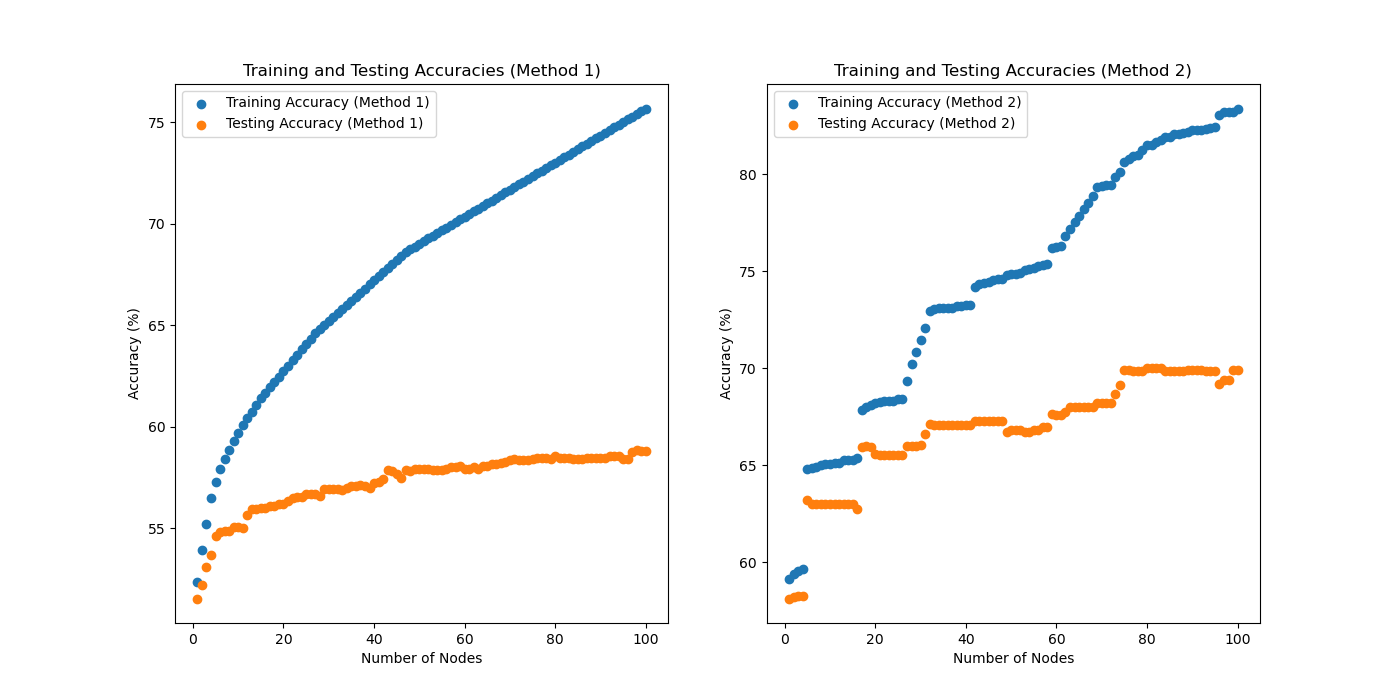
\includegraphics[width=\linewidth]{method_accuracies.png}
	\end{figure}
	
	\begin{figure}[H]
	\center
	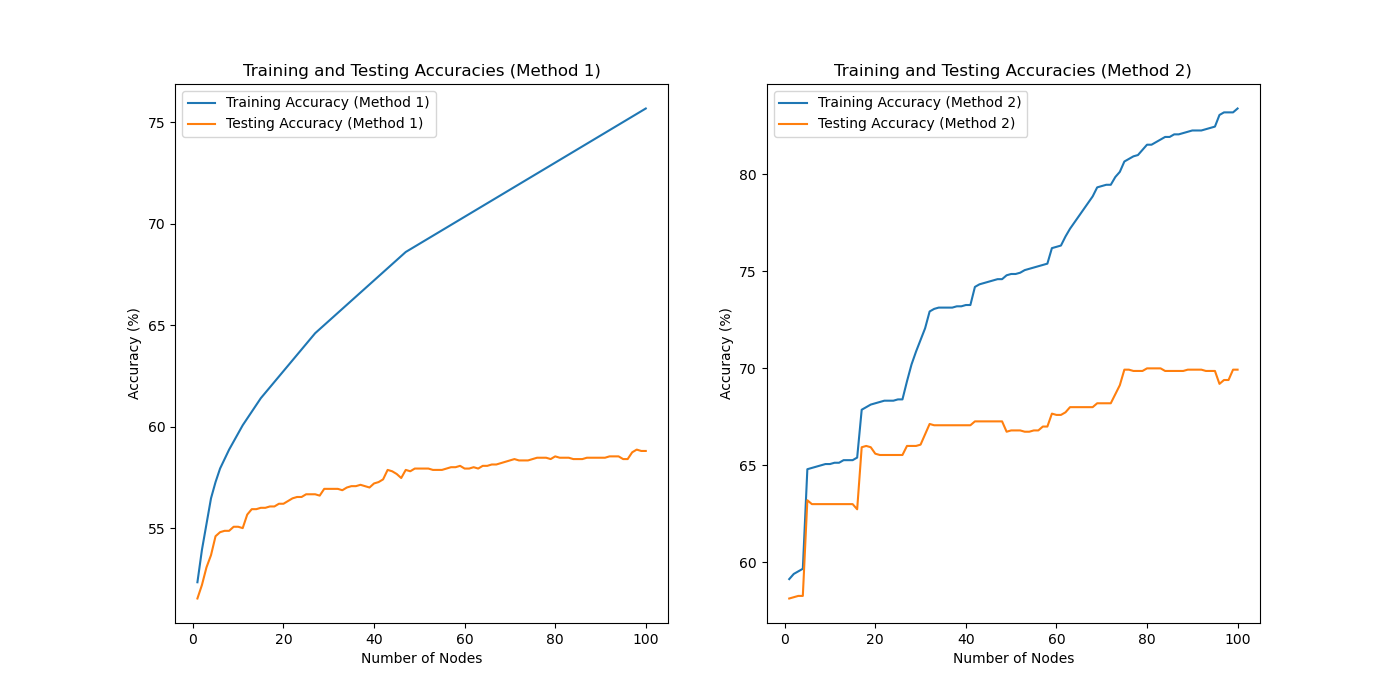
\includegraphics[width=\linewidth]{plot.png}
	\end{figure}
\end{enumerate}


%%%%%%%%%%%%%%%%%%%%%%%%%%%%%%%%%%%%%%%%%%%%%
%%%%%%%%%%%%%%%%%%%%%%%%%%%%%%%%%%%%%%%%%%%%%
\newpage
\subsection{} 
\begin{enumerate}
\part{a} 
	Bayes Network:
	
	\begin{figure}[H]
	\center
	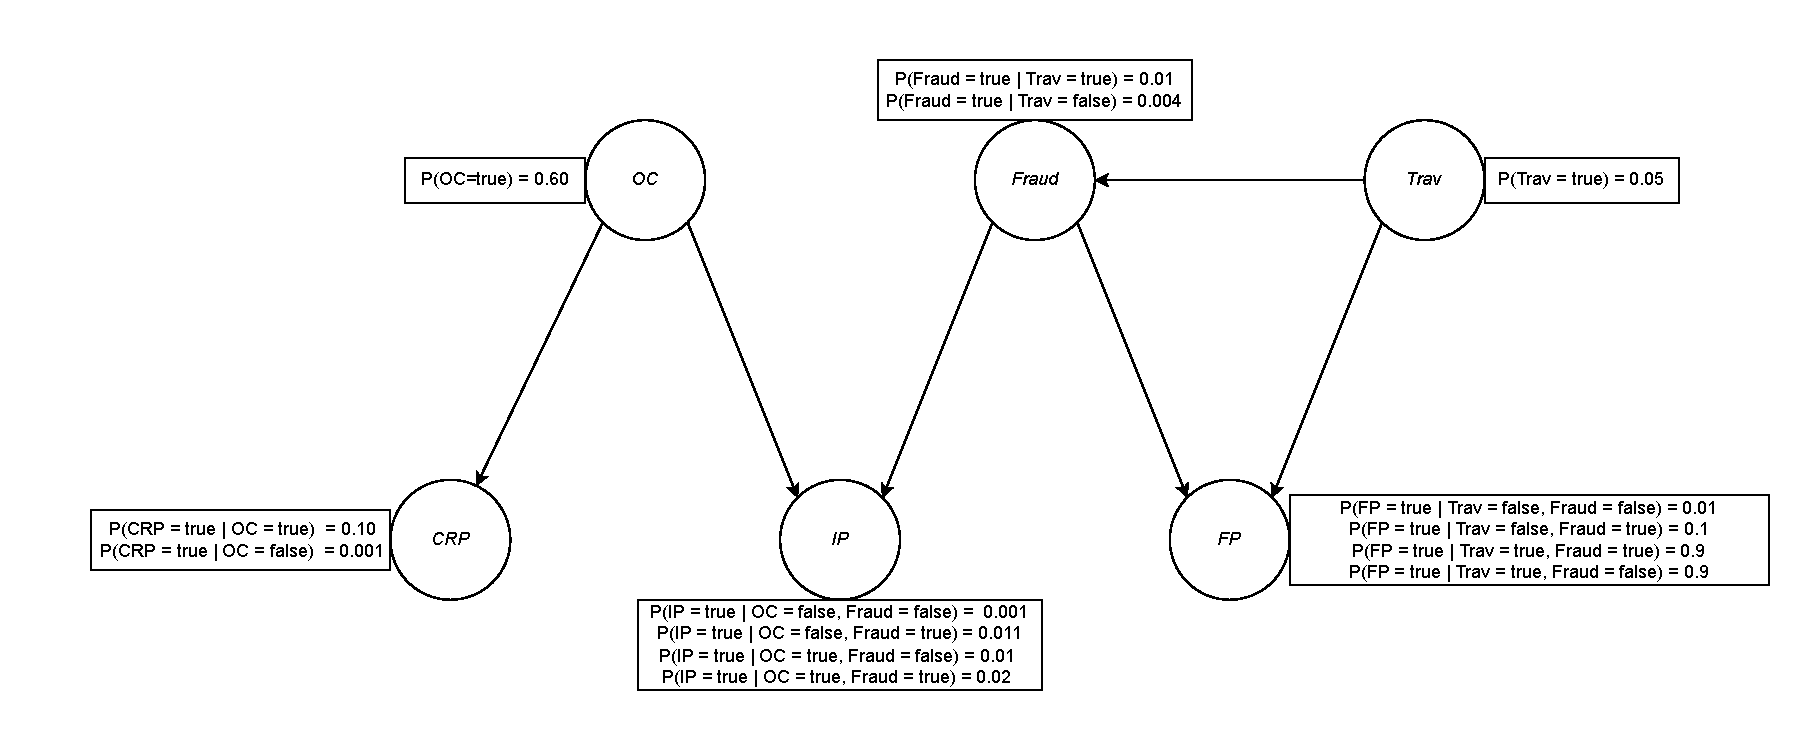
\includegraphics[ width=\linewidth]{486A2Q2a.pdf}
	\end{figure}
	
	\newpage
\part{b} 
	
	The prior probability that the current transaction is a fraud is:
	
	$P(Fraud=true) = \sum_{Trav}P(Fraud=true | Trav) P(Trav) $
	
	$= \sum_{Trav}f_1(Trav) f_0(Trav)$
	
	where $ f_0(Trav) = P(Trav)$ 
	\begin{tabular}{|c|c|}
	\hline
 	  $Trav$ & $f_0(Trav)$ \\
	\hline
	  $t$ & $ 0.05$  \\
	\hline
	  $f$ & $0.95$ \\
	\hline
	\end{tabular}
	
	where $f_1(Trav) = P(Fraud=true | Trav)$
	\begin{tabular}{|c|c|}
	\hline
 	  $Trav$ & $P(Fraud=true)$ \\
	\hline
	  $t$ & $ 0.01$  \\
	\hline
	  $f$ & $0.004$ \\
	\hline
	\end{tabular}
	
	Thus we get $P(Fraud=true) \propto \sum_{Trav}f_1(Trav) f_0(Trav)$
	
	$ = 0.05 \times 0.01 + 0.95 \times 0.004 = 0.0043$
	
	\noindent\rule[0.5ex]{\linewidth/2}{1pt}
	
	$f_0(Trav) = P(Trav) = $
	\begin{tabular}{|c|c|}
	\hline
 	  $Trav$ & $f_0(Trav)$ \\
	\hline
	  $t$ & $ 0.05$  \\
	\hline
	  $f$ & $0.95$ \\
	\hline
	\end{tabular}
	
	$f_1(Fraud, Trav) = P(Fraud | Trav) =$
	\begin{tabular}{|c|c|c|}
	\hline
 	  $Fraud$ & $Trav$ & $f_1(Fraud | Trav)$ \\
	\hline
	  $t$ & $t$ & $0.01$  \\
	\hline
	 $t$ & $f$ & $0.004$  \\
	\hline
	  $f$ & $t$ & $1 - 0.01 = 0.99$ \\
	\hline
	$f$ & $f$ & $1 - 0.004 = 0.996$  \\
	\hline
	\end{tabular}
	
	$f_2(OC) = P(OC) = $
	\begin{tabular}{|c|c|}
	\hline
 	  $OC$ & $f_2(OC)$ \\
	\hline
	  $t$ & $ 0.6$  \\
	\hline
	  $f$ & $0.4$ \\
	\hline
	\end{tabular}
	
	$f_3(Fraud, Trav) = P(FP = true | Fraud, Trav) = $
	\begin{tabular}{|c|c|c|}
	\hline
 	  $Fraud$ & $Trav$ & $f_3(Fraud, Trav)$ \\
	\hline
	  $t$ & $t$ & $0.9$  \\
	\hline
	 $t$ & $f$ & $0.1$  \\
	\hline
	  $f$ & $t$ & $0.9$ \\
	\hline
	$f$ & $f$ & $0.01$  \\
	\hline
	\end{tabular}
	
	$f_4(OC) = P(CRP = true | OC) = $
	\begin{tabular}{|c|c|}
	\hline
 	  $OC$ & $f_4(OC)$ \\
	\hline
	  $t$ & $ 0.1$  \\
	\hline
	  $f$ & $0.001$ \\
	\hline
	\end{tabular}
	
	$f_5(Fraud, OC) = P(IP = false | Fraud, OC) = $
	\begin{tabular}{|c|c|c|}
	\hline
 	  $Fraud$ & $OC$ & $f_5(Fraud, OC)$ \\
	\hline
	  $t$ & $t$ & $1 - 0.02 = 0.98$  \\
	\hline
	 $t$ & $f$ & $1 - 0.011 = 0.989$  \\
	\hline
	  $f$ & $t$ & $1 - 0.01 = 0.99$ \\
	\hline
	$f$ & $f$ & $1 - 0.001 = 0.999$  \\
	\hline
	\end{tabular}\\
	
	So that $P(Fraud | FP = true, IP = false, CRP = true)$
	
	$\propto \sum_{OC} \sum_{Trav} f_0(Trav) f_1(Fraud, Trav) f_2(OC) f_3(Fraud, Trav) f_4(OC) f_5(Fraud, OC)$
	
	$= \sum_{OC} f_2(OC) f_4(OC) f_5(Fraud, OC) \sum_{Trav} f_0(Trav) f_1(Fraud, Trav) f_3(Fraud, Trav)$
	
	$= \sum_{OC} f_2(OC) f_4(OC) f_5(Fraud, OC) f_6(Fraud)$\\
	
	Where $f_6(Fraud) = \sum_{Trav} f_0(Trav) f_1(Fraud, Trav) f_3(Fraud, Trav)$
	
	$=$
	\begin{tabular}{|c|c|}
	\hline
 	  $Fraud$ & $f_6(Fraud)$ \\
	\hline
	  $t$ & $0.05 \times 0.01 \times 0.9 + 0.95 \times 0.004 \times 0.1 = 0.00083$  \\
	\hline
	  $f$ & $0.05 \times 0.99 \times 0.9 + 0.95 \times 0.996 \times 0.01 = 0.054012 $ \\
	\hline
	\end{tabular}\\
	
	Then, we get $\sum_{OC} f_2(OC) f_4(OC) f_5(Fraud, OC) f_6(Fraud) = f_7(Fraud) f_6(fraud)$\\
	
	Where $f_7(Fraud) = \sum_{OC} f_2(OC) f_4(OC) f_5(Fraud, OC)$
	
	$=$
	\begin{tabular}{|c|c|}
	\hline
 	  $Fraud$ & $f_7(Fraud)$ \\
	\hline
	  $t$ & $0.6 \times 0.1 \times 0.98 + 0.4 \times 0.001 \times 0.989 = 0.0591956$  \\
	\hline
	  $f$ & $0.6 \times 0.1 \times 0.99 + 0.4 \times 0.001 \times 0.999 = 0.059799599999999994$ \\
	\hline
	\end{tabular}\\

	Thus, we get $f_8(Fraud) = f_7(Fraud) f_6(fraud)$
	
	$=$
	\begin{tabular}{|c|c|}
	\hline
 	  $Fraud$ & $f_8(Fraud)$ \\
	\hline
	  $t$ & $0.00083 \times 0.0591956 = 0.000049132348$  \\
	\hline
	  $f$ & $0.054012 \times 0.059799599999999994 = 0.0032298959951999997$ \\
	\hline
	\end{tabular}\\

	Thus, we get $P(Fraud  = true | FP = true, IP = false, CRP = true)$ as 
	
	$\frac{ 0.000049132348}{ 0.000049132348 +0.0032298959951999997 } = 0.014983813147541082 \approx 0.01498$
	
	\newpage
\part{c} 

	$f_0(Fraud) = P(Fraud | Trav = true) =$
	\begin{tabular}{|c|c|}
	\hline
 	  $Fraud$ & $f_0(Fraud)$ \\
	\hline
	  $t$ & $ 0.01 $  \\
	\hline
	  $f$ & $(1 - 0.01) = 0.99$ \\
	\hline
	\end{tabular}
	
	$f_1(OC) = P(OC) = $
	\begin{tabular}{|c|c|}
	\hline
 	  $OC$ & $f_1(OC)$ \\
	\hline
	  $t$ & $ 0.6$  \\
	\hline
	  $f$ & $0.4$ \\
	\hline
	\end{tabular}
	
	$f_2(Fraud) = P(FP = true | Fraud, Trav = true) = $
	\begin{tabular}{|c|c|}
	\hline
 	  $Fraud$ & $f_2(Fraud)$ \\
	\hline
	  $t$ & $ 0.9$  \\
	\hline
	  $f$ & $0.9$ \\
	\hline
	\end{tabular}
	
	$f_3(OC) = P(CRP = true | OC) = $
	\begin{tabular}{|c|c|}
	\hline
 	  $OC$ & $f_3(OC)$ \\
	\hline
	  $t$ & $ 0.1$  \\
	\hline
	  $f$ & $0.001$ \\
	\hline
	\end{tabular}
	
	$f_5(Fraud, OC) = P(IP = false | Fraud, OC) = $
	\begin{tabular}{|c|c|c|}
	\hline
 	  $Fraud$ & $OC$ & $f_5(Fraud, OC)$ \\
	\hline
	  $t$ & $t$ & $1 - 0.02 = 0.98$  \\
	\hline
	 $t$ & $f$ & $1 - 0.011 = 0.989$  \\
	\hline
	  $f$ & $t$ & $1 - 0.01 = 0.99$ \\
	\hline
	$f$ & $f$ & $1 - 0.001 = 0.999$  \\
	\hline
	\end{tabular}\\

	So, $P(Fraud | FP = true, IP = false, CRP = true, Trav = true)$
	
	$= \sum_{OC}f_0(Fraud)f_1(OC)f_2(Fraud)f_3(OC)f_5(Fraud, OC) $
	
	$= f_0(Fraud)f_2(Fraud)\sum_{OC}f_1(OC)f_3(OC)f_5(Fraud, OC)$
	
	$= f_0(Fraud)f_2(Fraud)f_6(Fraud)$\\
	
	Where $f_6(Fraud) = \sum_{OC}f_1(OC)f_3(OC)f_5(Fraud, OC)$
	
	$=$
	\begin{tabular}{|c|c|}
	\hline
 	  $Fraud$ & $f_6(Fraud)$ \\
	\hline
	  $t$ & $0.6 \times 0.1 \times 0.98 + 0.4 \times 0.001 \times 0.989 = 0.0591956$  \\
	\hline
	  $f$ & $0.6 \times 0.1 \times 0.99 + 0.4 \times 0.001 \times 0.999 = 0.0597996$ \\
	\hline
	\end{tabular}\\
	
	Thus, we get $f_7(Fraud) = f_0(Fraud)f_2(Fraud)f_6(Fraud)$
	
	$=$
	\begin{tabular}{|c|c|}
	\hline
 	  $Fraud$ & $f_7(Fraud)$ \\
	\hline
	  $t$ & $0.01 \times 0.9 \times 0.0591956 = 0.0005327604$  \\
	\hline
	  $f$ & $0.99 \times 0.9 \times 0.0597996 = 0.0532814436$ \\
	\hline
	\end{tabular}\\
	
	Thus, we get $P(Fraud = true | FP = true, IP = false, CRP = true, Trav = true)$
	
	$= \frac{0.0005327604}{0.0005327604 + 0.0532814436} = 0.00989999591929298 \approx 0.0099$
	
	\newpage
\part{d}

	We will need to calculate $P(Fraud | IP = true)$.
	
	$f_0(Trav) = P(Trav) = $
	\begin{tabular}{|c|c|}
	\hline
 	  $Trav$ & $f_0(Trav)$ \\
	\hline
	  $t$ & $ 0.05$  \\
	\hline
	  $f$ & $0.95$ \\
	\hline
	\end{tabular}

	$f_1(Fraud, Trav) = P(Fraud | Trav) =$
	\begin{tabular}{|c|c|c|}
	\hline
 	  $Fraud$ & $Trav$ & $f_1(Fraud | Trav)$ \\
	\hline
	  $t$ & $t$ & $0.01$  \\
	\hline
	 $t$ & $f$ & $0.004$  \\
	\hline
	  $f$ & $t$ & $1 - 0.01 = 0.99$ \\
	\hline
	$f$ & $f$ & $1 - 0.004 = 0.996$  \\
	\hline
	\end{tabular}
	
	$f_2(OC) = P(OC) = $
	\begin{tabular}{|c|c|}
	\hline
 	  $OC$ & $f_2(OC)$ \\
	\hline
	  $t$ & $ 0.6$  \\
	\hline
	  $f$ & $0.4$ \\
	\hline
	\end{tabular}
	
	$f_3(FP, Fraud, Trav) = P(FP | Fraud, Trav) = $
	\begin{tabular}{|c|c|c|c|}
	\hline
 	  $FP$ & $Fraud$ & $Trav$ & $f_3(Fraud, Trav)$ \\
 	  \hline
	  $t$ & $t$ & $t$ & $0.9$\\
	  \hline
	  $t$ & $t$ & $f$ & $0.1$\\
	  \hline
	  $t$ & $f$ & $t$ & $0.9$\\
	  \hline
	  $t$ & $f$ & $f$ & $0.01$\\
	  \hline
	  $f$ & $t$ & $t$ & $1 - 0.9 = 0.1$\\
	  \hline
	  $f$ & $t$ & $f$ & $1 - 0.1 = 0.9$\\
	  \hline
	  $f$ & $f$ & $t$ & $1 - 0.9 = 0.1$\\
	  \hline
	  $f$ & $f$ & $f$ & $1 - 0.01 = 0.99$\\
	  \hline
	\end{tabular}
	
	$f_4(CRP, OC) = P(CRP | OC) = $
	\begin{tabular}{|c|c|c|}
	\hline
 	  $CRP$ & $OC$ & $f_4(CRP, OC))$ \\
	\hline
	  $t$ & $t$ & $0.10$  \\
	\hline
	 $t$ & $f$ & $0.001$  \\
	\hline
	 $f$ & $t$ & $1 - 0.10 = 0.9$ \\
	\hline
	$f$ & $f$ & $1 - 0.001 = 0.999$  \\
	\hline
	\end{tabular}
	
	$f_5(Fraud, OC) = P(IP = true | Fraud, OC) = $
	\begin{tabular}{|c|c|c|}
	\hline
 	  $Fraud$ & $OC$ & $f_5(Fraud, OC)$ \\
	\hline
	  $t$ & $t$ & $0.02$  \\
	\hline
	 $t$ & $f$ & $0.011$  \\
	\hline
	  $f$ & $t$ & $0.01$ \\
	\hline
	$f$ & $f$ & $0.001$  \\
	\hline
	\end{tabular}\\
	
	Thus we get $P(Fraud | IP = true)$
	
	$\propto \sum_{CRP} \sum_{OC} f_2(OC) f_4(CRP, OC) f_5(Fraud, OC) \sum_{FP} \sum_{Trav} f_0(Trav) f_1(Fraud, Trav) f_3(FP, Fraud, Trav)$
	
	$= \sum_{CRP} \sum_{OC} f_2(OC) f_4(CRP, OC) f_5(Fraud, OC) \sum_{FP} f_6(Fraud, FP)$\\
	
	Where $f_6(Fraud, FP) = \sum_{Trav} f_0(Trav) f_1(Fraud, Trav) f_3(FP, Fraud, Trav)$
	
	$=$
	\begin{tabular}{|c|c|c|}
	\hline
 	  $Fraud$ & $FP$ & $f_6(Fraud, FP)$ \\
	\hline
	  $t$ & $t$ & $0.05 \times 0.01 \times 0.9 + 0.95 \times 0.004 \times 0.1 = 0.00083$  \\
	\hline
	 $t$ & $f$ & $0.05 \times 0.01 \times 0.1 + 0.95 \times 0.004 \times 0.9 = 0.00347$  \\
	\hline
	  $f$ & $t$ & $0.05 \times 0.99 \times 0.9 + 0.95 \times 0.996 \times 0.01 = 0.054012 $ \\
	\hline
	$f$ & $f$ & $0.05 \times 0.99 \times 0.1 + 0.95 \times 0.996 \times 0.99 = 0.941688 $  \\
	\hline
	\end{tabular}\\	
		
	So, $\sum_{CRP} \sum_{OC} f_2(OC) f_4(CRP, OC) f_5(Fraud, OC) \sum_{FP} f_6(Fraud, FP)$
	
	$= \sum_{CRP} \sum_{OC} f_2(OC) f_4(CRP, OC) f_5(Fraud, OC) f_7(Fraud)$\\
	
	Where $f_7(Fraud) = \sum_{FP} f_6(Fraud, FP)$
	
	\begin{tabular}{|c|c|}
	\hline
 	  $Fraud$ & $f_7(Fraud)$ \\
	\hline
	  $t$ & $ 0.00083 + 0.00347 = 0.0043$  \\
	\hline
	  $f$ & $ 0.054012 + 0.941688 = 0.9957$ \\
	\hline
	\end{tabular}\\
	
	So, $\sum_{CRP} \sum_{OC} f_2(OC) f_4(CRP, OC) f_5(Fraud, OC) f_7(Fraud) = \sum_{CRP} f_{8}(Fraud, CRP)$\\
	
	Where $f_8(Fraud, CRP) = \sum_{OC} f_2(OC) f_4(CRP, OC) f_5(Fraud, OC) f_7(Fraud)$
	
	$=$
	\begin{tabular}{|c|c|c|}
	\hline
 	  $Fraud$ & $CRP$ & $f_8(Fraud, CRP)$ \\
	\hline
	  $t$ & $t$ & $0.6 \times 0.1 \times 0.02 \times 0.0043 + 0.4 \times 0.001 \times 0.011 \times 0.0043 = 0.00000517892$  \\
	\hline
	 $t$ & $f$ & $0.6 \times 0.9 \times 0.02 \times 0.0043 + 0.4 \times 0.999 \times 0.011 \times 0.0043 = 0.00006534108$  \\
	\hline
	  $f$ & $t$ & $0.6 \times 0.1 \times 0.01 \times 0.9957 + 0.4 \times 0.001 \times 0.001 \times 0.9957 = 0.00059781828$ \\
	\hline
	$f$ & $f$ & $0.6 \times 0.9 \times 0.01 \times 0.9957 + 0.4 \times 0.999 \times 0.001 \times 0.9957 = 0.00577466172$  \\
	\hline
	\end{tabular}\\	
	
	So, $f_9(Fraud) = \sum_{CRP} f_{8}(Fraud, CRP)$
	
	$=$
	\begin{tabular}{|c|c|}
	\hline
 	  $Fraud$ & $f_9(Fraud)$ \\
	\hline
	  $t$ & $ 0.00000517892 + 0.00006534108 = 0.00007052$  \\
	\hline
	  $f$ & $ 0.00059781828 + 0.00577466172 = 0.00637248$ \\
	\hline
	\end{tabular}
	
	So, we get $P(Fraud = true | IP = true) = \frac{0.00007052}{0.00007052 + 0.00637248} = 0.010945211857830203 \approx 0.01095$.
	
	\noindent\rule[0.5ex]{\linewidth/2}{1pt}
	
	Now we proceed with $P(Fraud = true | IP = true, CRP = true)$:
	
	$f_0(Trav) = P(Trav) = $
	\begin{tabular}{|c|c|}
	\hline
 	  $Trav$ & $f_0(Trav)$ \\
	\hline
	  $t$ & $ 0.05$  \\
	\hline
	  $f$ & $0.95$ \\
	\hline
	\end{tabular}

	$f_1(Fraud, Trav) = P(Fraud | Trav) =$
	\begin{tabular}{|c|c|c|}
	\hline
 	  $Fraud$ & $Trav$ & $f_1(Fraud | Trav)$ \\
	\hline
	  $t$ & $t$ & $0.01$  \\
	\hline
	 $t$ & $f$ & $0.004$  \\
	\hline
	  $f$ & $t$ & $1 - 0.01 = 0.99$ \\
	\hline
	$f$ & $f$ & $1 - 0.004 = 0.996$  \\
	\hline
	\end{tabular}
	
	$f_2(OC) = P(OC) = $
	\begin{tabular}{|c|c|}
	\hline
 	  $OC$ & $f_2(OC)$ \\
	\hline
	  $t$ & $ 0.6$  \\
	\hline
	  $f$ & $0.4$ \\
	\hline
	\end{tabular}
	
	$f_3(FP, Fraud, Trav) = P(FP | Fraud, Trav) = $
	\begin{tabular}{|c|c|c|c|}
	\hline
 	  $FP$ & $Fraud$ & $Trav$ & $f_3(Fraud, Trav)$ \\
 	  \hline
	  $t$ & $t$ & $t$ & $0.9$\\
	  \hline
	  $t$ & $t$ & $f$ & $0.1$\\
	  \hline
	  $t$ & $f$ & $t$ & $0.9$\\
	  \hline
	  $t$ & $f$ & $f$ & $0.01$\\
	  \hline
	  $f$ & $t$ & $t$ & $1 - 0.9 = 0.1$\\
	  \hline
	  $f$ & $t$ & $f$ & $1 - 0.1 = 0.9$\\
	  \hline
	  $f$ & $f$ & $t$ & $1 - 0.9 = 0.1$\\
	  \hline
	  $f$ & $f$ & $f$ & $1 - 0.01 = 0.99$\\
	  \hline
	\end{tabular}
	
	$f_4(OC) = P(CRP = true | OC) = $
	\begin{tabular}{|c|c|c|}
	\hline
 	  $OC$ & $f_4(OC))$ \\
	\hline
	  $t$ & $0.10$  \\
	\hline
	 $f$ & $0.001$  \\
	\hline
	\end{tabular}
	
	$f_5(Fraud, OC) = P(IP = true | Fraud, OC) = $
	\begin{tabular}{|c|c|c|}
	\hline
 	  $Fraud$ & $OC$ & $f_5(Fraud, OC)$ \\
	\hline
	  $t$ & $t$ & $0.02$  \\
	\hline
	 $t$ & $f$ & $0.011$  \\
	\hline
	  $f$ & $t$ & $0.01$ \\
	\hline
	$f$ & $f$ & $0.001$  \\
	\hline
	\end{tabular}\\
	
	Thus we get $P(Fraud | IP = true, CRP = true)$
	
	$\propto \sum_{OC} f_2(OC) f_4(OC) f_5(Fraud, OC) \sum_{FP} \sum_{Trav} f_0(Trav) f_1(Fraud, Trav) f_3(FP, Fraud, Trav)$
	
	$= \sum_{OC} f_2(OC) f_4(OC) f_5(Fraud, OC) \sum_{FP} f_6(Fraud, FP)$\\
	
	Where $f_6(Fraud, FP) = \sum_{Trav} f_0(Trav) f_1(Fraud, Trav) f_3(FP, Fraud, Trav)$
	
	$=$
	\begin{tabular}{|c|c|c|}
	\hline
 	  $Fraud$ & $FP$ & $f_6(Fraud, FP)$ \\
	\hline
	  $t$ & $t$ & $0.05 \times 0.01 \times 0.9 + 0.95 \times 0.004 \times 0.1 = 0.00083$  \\
	\hline
	 $t$ & $f$ & $0.05 \times 0.01 \times 0.1 + 0.95 \times 0.004 \times 0.9 = 0.00347$  \\
	\hline
	  $f$ & $t$ & $0.05 \times 0.99 \times 0.9 + 0.95 \times 0.996 \times 0.01 = 0.054012 $ \\
	\hline
	$f$ & $f$ & $0.05 \times 0.99 \times 0.1 + 0.95 \times 0.996 \times 0.99 = 0.941688 $  \\
	\hline
	\end{tabular}\\	
		
	So, $ \sum_{OC} f_2(OC) f_4(OC) f_5(Fraud, OC) \sum_{FP} f_6(Fraud, FP)$
	
	$= \sum_{OC} f_2(OC) f_4(OC) f_5(Fraud, OC) f_7(Fraud)$\\
	
	Where $f_7(Fraud) = \sum_{FP} f_6(Fraud, FP)$
	
	\begin{tabular}{|c|c|}
	\hline
 	  $Fraud$ & $f_7(Fraud)$ \\
	\hline
	  $t$ & $ 0.00083 + 0.00347 = 0.0043$  \\
	\hline
	  $f$ & $ 0.054012 + 0.941688 = 0.9957$ \\
	\hline
	\end{tabular}\\
	
	So, $\sum_{OC} f_2(OC) f_4(OC) f_5(Fraud, OC) f_7(Fraud) = f_{8}(Fraud)$\\

	$=$
	\begin{tabular}{|c|c|c|}
	\hline
 	  $Fraud$ & $f_8(Fraud)$ \\
	\hline
	  $t$ & $0.6 \times 0.1 \times 0.02 \times 0.0043 + 0.4 \times 0.001 \times 0.011 \times 0.0043 = 0.00000517892$  \\
	\hline
	  $f$ & $0.6 \times 0.1 \times 0.01 \times 0.9957 + 0.4 \times 0.001 \times 0.001 \times 0.9957 = 0.00059781828$ \\
	\hline
	\end{tabular}\\	
	
	So, we get $P(Fraud = true | IP = true, CRP = true) = \frac{0.00000517892}{0.00000517892 + 0.00059781828} = 0.008588630262296408$
	
	$\approx 0.00859$.
	
	So by having $CRP = true$ prior to my internet purchase, the chance of the transaction being rejected as a possible fraud is reduced by $0.010945211857830203 - 0.008588630262296408 = 0.00235658 \approx 0.00236$. 
\end{enumerate}

%%%%%%%%%%%%%%%%%%%%%%%%%%%%%%%%%%%%%%%%%%%%%
%%%%%%%%%%%%%%%%%%%%%%%%%%%%%%%%%%%%%%%%%%%%%

\iffalse
	
	$f_0() = P(Fraud = True) = 0.0043$\footnote{From previous calculation}
	
	$f_1(Trav) = P(Trav)$ 
	\begin{tabular}{|c|c|}
	\hline
 	  $Trav$ & $f_1(Trav)$ \\
	\hline
	  $t$ & $ 0.05$  \\
	\hline
	  $f$ & $0.95$ \\
	\hline
	\end{tabular}
	
	$f_2(OC) = P(OC)$
	\begin{tabular}{|c|c|}
	\hline
 	  $OC$ & $f_2(OC)$ \\
	\hline
	  $t$ & $ 0.6$  \\
	\hline
	  $f$ & $0.4$ \\
	\hline
	\end{tabular}
	
	$f_3(Trav) = P(FP = true | Fraud = true, Trav)$
	\begin{tabular}{|c|c|}
	\hline
 	  $Trav$ & $f_3(Trav)$ \\
	\hline
	  $t$ & $ 0.9$  \\
	\hline
	  $f$ & $0.1$ \\
	\hline
	\end{tabular}
	
	
	$f_4(OC) = P(CRP = true | OC)$
	\begin{tabular}{|c|c|}
	\hline
 	  $OC$ & $f_4(OC)$ \\
	\hline
	  $t$ & $ 0.1$  \\
	\hline
	  $f$ & $0.001$ \\
	\hline
	\end{tabular}
	
	$f_5(OC) = P(IP = false | Fraud = true, OC)$
	\begin{tabular}{|c|c|}
	\hline
 	  $OC$ & $f_5(OC)$ \\
	\hline
	  $t$ & $ 1 - 0.02 = 0.98$  \\
	\hline
	  $f$ & $ 1 - 0.011 = 0.989$ \\
	\hline
	\end{tabular}\\
	
	
	So that $P(Fraud = true | FP = true, IP = false, CRP = true)$
	
	$\propto \sum_{CRP} \sum_{OC} \sum_{IP} \sum_{Fraud} \sum_{FP} \sum_{Trav} f_0() f_1(Trav) f_2(OC) f_3(Trav) f_4(OC) f_5(OC)$
	
	$= \sum_{OC}f_2(OC) f_4(OC) f_5(OC) \sum_{Trav}f_0() f_1(Trav) f_3(Trav)$
	
	$= \sum_{OC}f_2(OC) f_4(OC) f_5(OC) f_6()$\\
	
	Where $f_6() = \sum_{Trav}f_0() f_1(Trav) f_3(Trav) = 0.0043 \times 0.9 \times 0.05 + 0.0043 \times 0.95 \times 0.1 = 0.000602$
	
	= $f_7() \times 0.000602$
	
	Where $f_7() = \sum_{OC}f_2(OC) f_4(OC) f_5(OC) = 0.98 \times 0.1 \times 0.6 + 0.989 \times 0.001 \times 0.4 = 0.0591956$
	
	$= 0.0591956 \times 0.000602$
	
	$= 0.00003563575$
	
	Thus we get $P(Fraud = true | FP = true, IP = false, CRP = true) = 0.00003563575$. \\
	
	Now let's compute $P(Fraud = false | FP = true, IP = false, CRP = true)$.
	
	We will redefine the following terms while keep the rest same:
	
	$f_0() = P(Fraud = True) = 1 - 0.0043 = 0.9957$
	
	$f_3(Trav) = P(FP = true | Fraud = false, Trav)$
	\begin{tabular}{|c|c|}
	\hline
 	  $Trav$ & $f_3(Trav)$ \\
	\hline
	  $t$ & $ 0.9$  \\
	\hline
	  $f$ & $0.01$ \\
	\hline
	\end{tabular}
	
	$f_5(OC) = P(IP = false | Fraud = false, OC)$
	\begin{tabular}{|c|c|}
	\hline
 	  $OC$ & $f_5(OC)$ \\
	\hline
	  $t$ & $ 1 - 0.01 = 0.99$  \\
	\hline
	  $f$ & $ 1 - 0.001 = 0.999$ \\
	\hline
	\end{tabular}\\
	
	So we get $P(Fraud = false | FP = true, IP = false, CRP = true)$
	
	$\propto \sum_{CRP} \sum_{OC} \sum_{IP} \sum_{Fraud} \sum_{FP} \sum_{Trav} f_0() f_1(Trav) f_2(OC) f_3(Trav) f_4(OC) f_5(OC)$
	
	$= \sum_{OC}f_2(OC) f_4(OC) f_5(OC) \sum_{Trav}f_0() f_1(Trav) f_3(Trav)$
	
	$= \sum_{OC}f_2(OC) f_4(OC) f_5(OC) f_6()$\\
	
	Where $f_6() = \sum_{Trav}f_0() f_1(Trav) f_3(Trav) = 0.9957 \times 0.05 \times 0.9 + 0.9957 \times 0.95 \times 0.01 = 0.05426565$
	
	$= f_7() \times 0.0139398$
	
	Where $f_7() = \sum_{OC}f_2(OC) f_4(OC) f_5(OC) = 0.99 \times 0.1 \times 0.6 + 0.999 \times 0.001 \times 0.4 = 0.0597996$
	
	$ = 0.0597996 \times 0.05426565 $
	
	$ = 0.00324506416374$
	
	Thus we can now normalize $P(Fraud = true | FP = true, IP = false, CRP = true)$
	
	$ = \frac{0.00003563575}{0.00003563575 + 0.00324506416374}$
	
	$\approx 0.01086224$
	
	\fi
	
	\iffalse
	
	$f_0() = P(Fraud = True) = 0.0043$\footnote{From previous calculation}
	
	$f_1(Trav) = P(Trav)$ 
	\begin{tabular}{|c|c|}
	\hline
 	  $Trav$ & $f_1(Trav)$ \\
	\hline
	  $t$ & $ 0.05$  \\
	\hline
	  $f$ & $0.95$ \\
	\hline
	\end{tabular}
	
	$f_2(OC) = P(OC)$
	\begin{tabular}{|c|c|}
	\hline
 	  $OC$ & $f_2(OC)$ \\
	\hline
	  $t$ & $ 0.6$  \\
	\hline
	  $f$ & $0.4$ \\
	\hline
	\end{tabular}
	
	$f_3(Trav) = P(FP = true | Fraud = true, Trav)$
	\begin{tabular}{|c|c|}
	\hline
 	  $Trav$ & $f_3(Trav)$ \\
	\hline
	  $t$ & $ 0.9$  \\
	\hline
	  $f$ & $0.1$ \\
	\hline
	\end{tabular}
	
	
	$f_4(OC) = P(CRP = true | OC)$
	\begin{tabular}{|c|c|}
	\hline
 	  $OC$ & $f_4(OC)$ \\
	\hline
	  $t$ & $ 0.1$  \\
	\hline
	  $f$ & $0.001$ \\
	\hline
	\end{tabular}
	
	$f_5(OC) = P(IP = false | Fraud = true, OC)$
	\begin{tabular}{|c|c|}
	\hline
 	  $OC$ & $f_5(OC)$ \\
	\hline
	  $t$ & $ 0.98$  \\
	\hline
	  $f$ & $0.989$ \\
	\hline
	\end{tabular}\\
	
	
	So that $P(Fraud = true | FP = true, IP = false, CRP = true)$
	
	$\propto \sum_{OC, Trav} f_0() f_1(Trav) f_2(OC) f_3(Trav) f_4(OC) f_5(OC)$
	
	$= \sum_{OC}f_2(OC) f_4(OC) f_5(OC) \sum_{Trav}f_0() f_1(Trav) f_3(Trav)$
	
	$= f_6() f_7()$\\
	
	
	Where $f_6() = \sum_{OC}f_2(OC) f_4(OC) f_5(OC)$
	
	$= 0.98 \times 0.1 \times 0.6 + 0.989 \times 0.001 \times 0.4 = 0.0591956$
	
	
	And $f_7() = \sum_{Trav}f_0() f_1(Trav) f_3(Trav)$
	
	$= 0.0043 \times 0.9 \times 0.05 + 0.0043 \times 0.95 \times 0.1 = 0.000602$
	
	So, we get $P(Fraud = true | FP = true, IP = false, CRP = true)$
	
	$= 0.0591956 \times 0.000602 = 0.00003563575$
	
	\fi

\end{document}
